\begin{figure}[!]
    \centering
    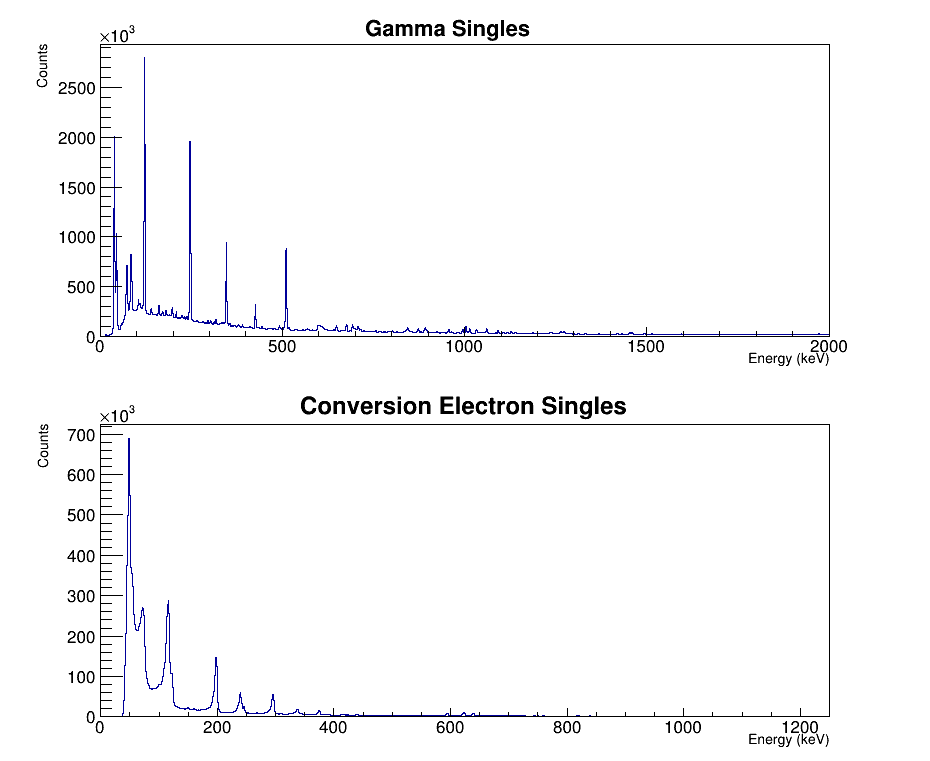
\includegraphics[scale=0.4]{154GdTablesAndFigs/154Gd_Singles.png}
    \caption{Singles spectra of $^{154}$Gd. In the $\gamma$ spectrum on top, several lines stand out prominently. These are the ground-state band lines. In the conversion electron spectrum on the bottom, the large peaks up to approximately 450 keV are from the ground state band. These large peaks make the ground state band a good diagnostic, but also emphasize the need for coincidence gating, as the conversion electron spectrum is flooded by the ground state band electrons. The large peak at low energy is cut off due to the threshold. It is a combination of background and the 123K peak.}
    \label{fig:154Gd_Singles}
\end{figure}